\documentclass{standalone}
\usepackage{tikz}
\usetikzlibrary{patterns, positioning}
\usepackage[sfdefault]{ClearSans} %% option 'sfdefault' activates Clear Sans as the default text font
\usepackage[T1]{fontenc}

\begin{document}
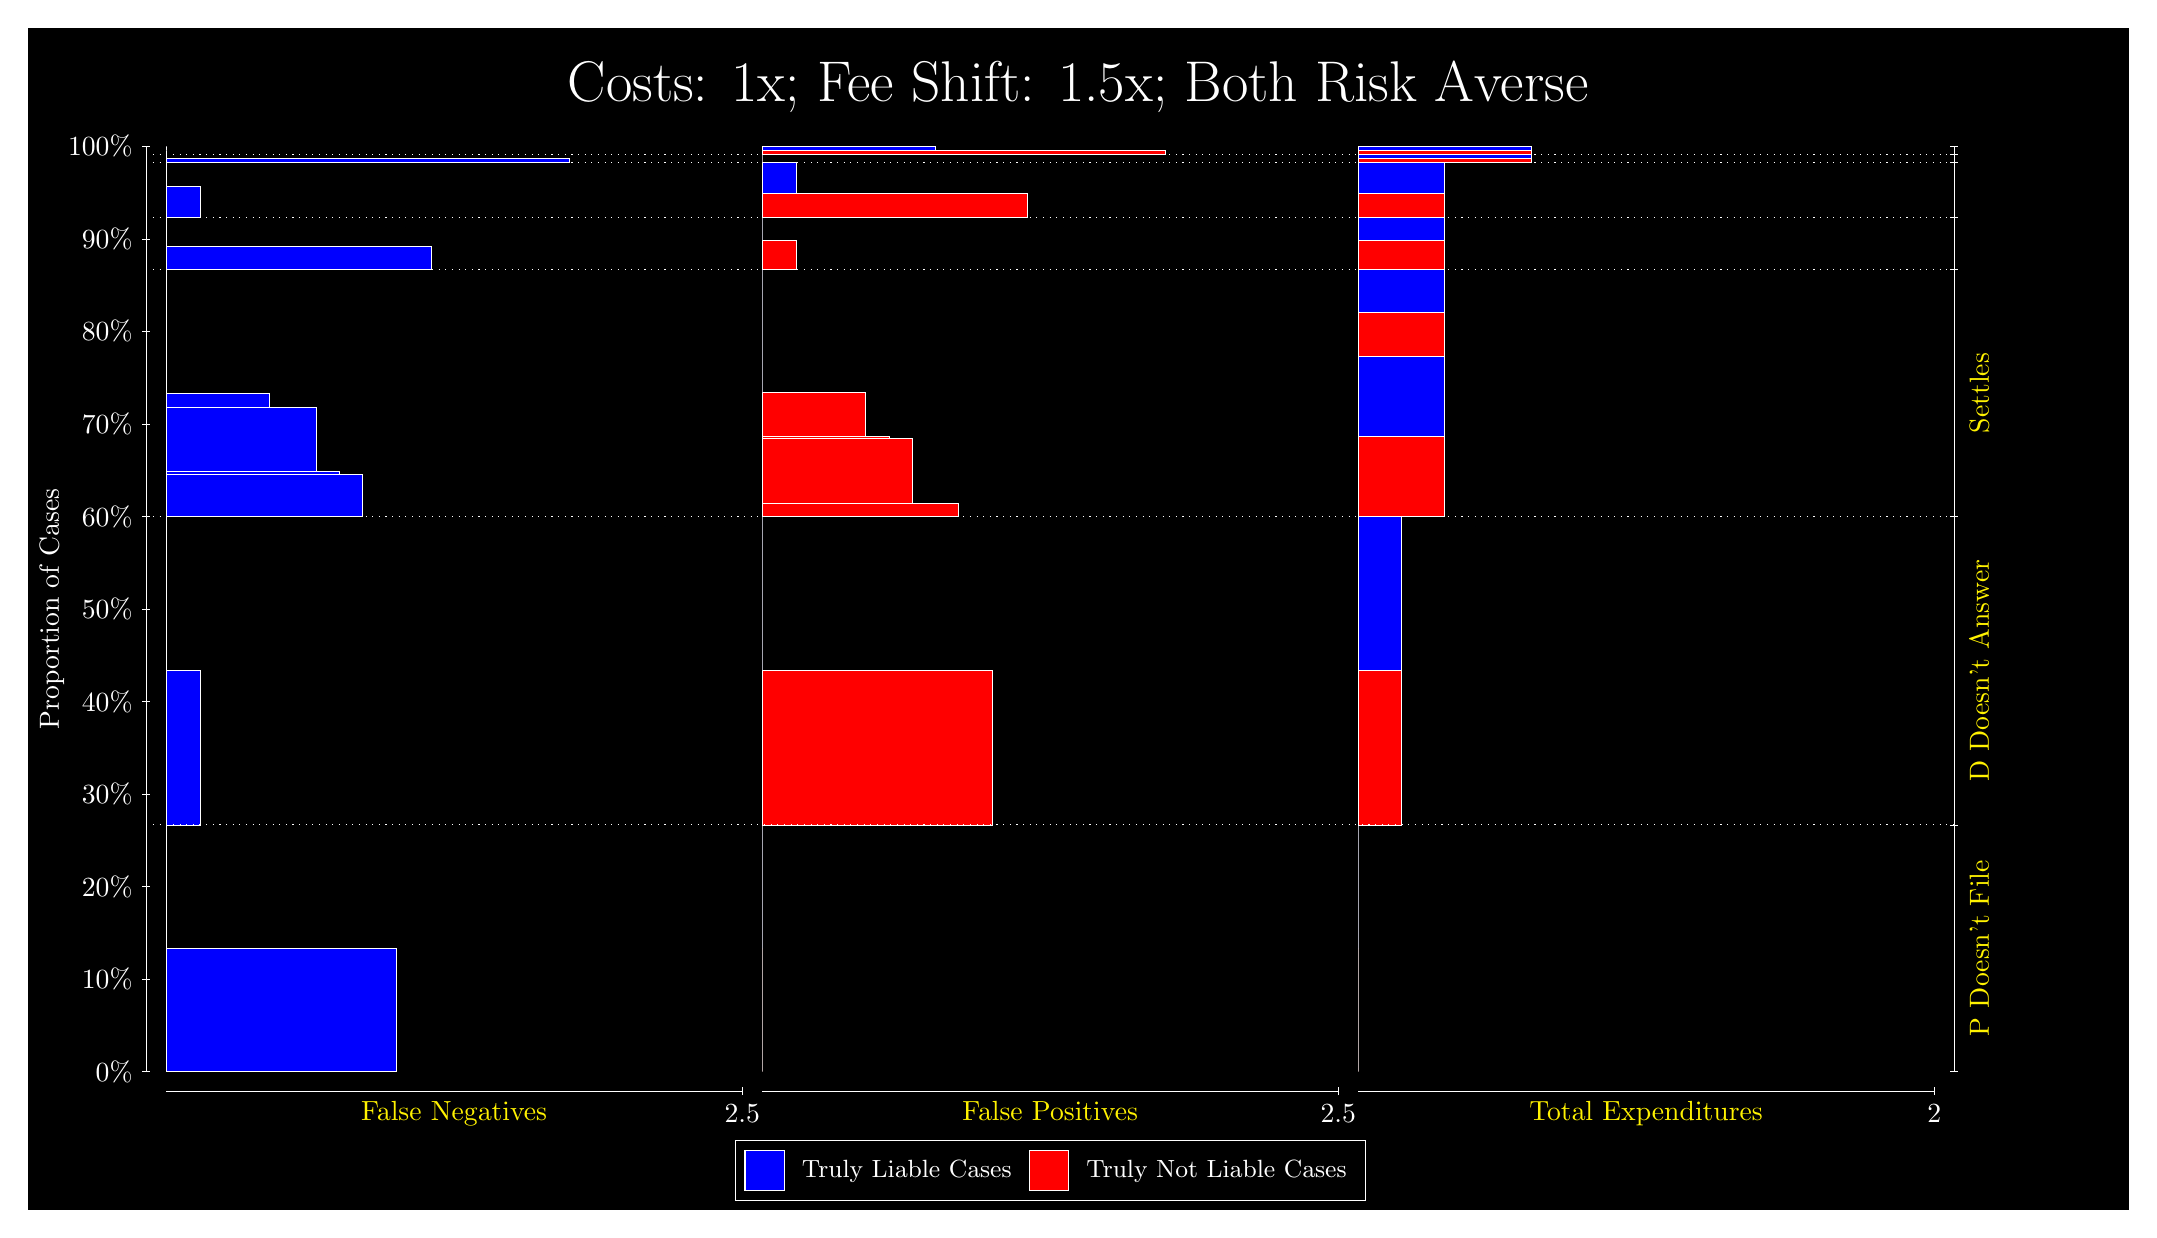
\begin{tikzpicture}
\draw[fill=black] (0,0) rectangle (26.667,15);
\draw[text=white] (0,13.5) rectangle (26.667,15) node[midway] {\huge Costs: 1x; Fee Shift: 1.5x; Both Risk Averse};
\draw[white, very thin] (1.5,1.75) -- (1.5,13.5);
\node[rotate=90, text=white, anchor=center] at (0.3, 7.625) {Proportion of Cases};
\draw[white, very thin] (1.45,1.75) -- (1.55,1.75);
\node[text=white, anchor=east] at (1.45, 1.75) {0\%};
\draw[white, very thin] (1.45,2.925) -- (1.55,2.925);
\node[text=white, anchor=east] at (1.45, 2.925) {10\%};
\draw[white, very thin] (1.45,4.1) -- (1.55,4.1);
\node[text=white, anchor=east] at (1.45, 4.1) {20\%};
\draw[white, very thin] (1.45,5.275) -- (1.55,5.275);
\node[text=white, anchor=east] at (1.45, 5.275) {30\%};
\draw[white, very thin] (1.45,6.45) -- (1.55,6.45);
\node[text=white, anchor=east] at (1.45, 6.45) {40\%};
\draw[white, very thin] (1.45,7.625) -- (1.55,7.625);
\node[text=white, anchor=east] at (1.45, 7.625) {50\%};
\draw[white, very thin] (1.45,8.8) -- (1.55,8.8);
\node[text=white, anchor=east] at (1.45, 8.8) {60\%};
\draw[white, very thin] (1.45,9.975) -- (1.55,9.975);
\node[text=white, anchor=east] at (1.45, 9.975) {70\%};
\draw[white, very thin] (1.45,11.15) -- (1.55,11.15);
\node[text=white, anchor=east] at (1.45, 11.15) {80\%};
\draw[white, very thin] (1.45,12.325) -- (1.55,12.325);
\node[text=white, anchor=east] at (1.45, 12.325) {90\%};
\draw[white, very thin] (1.45,13.5) -- (1.55,13.5);
\node[text=white, anchor=east] at (1.45, 13.5) {100\%};

\draw[white, very thin] (24.457,1.75) -- (24.457,13.5);
\draw[white, very thin] (24.407,1.75) -- (24.507,1.75);
\node[anchor=west] at (24.407, 1.75) {};
\draw[white, very thin] (24.407,4.8833) -- (24.507,4.8833);
\node[anchor=west] at (24.407, 4.8833) {};
\draw[white, very thin] (24.407,8.8) -- (24.507,8.8);
\node[anchor=west] at (24.407, 8.8) {};
\draw[white, very thin] (24.407,11.935) -- (24.507,11.935);
\node[anchor=west] at (24.407, 11.935) {};
\draw[white, very thin] (24.407,12.601) -- (24.507,12.601);
\node[anchor=west] at (24.407, 12.601) {};
\draw[white, very thin] (24.407,13.295) -- (24.507,13.295);
\node[anchor=west] at (24.407, 13.295) {};
\draw[white, very thin] (24.407,13.398) -- (24.507,13.398);
\node[anchor=west] at (24.407, 13.398) {};
\draw[white, very thin] (24.407,13.5) -- (24.507,13.5);
\node[anchor=west] at (24.407, 13.5) {};

\draw[white, very thin, fill=blue] (1.75,1.75) rectangle (4.6775,3.3167);
\draw[white, very thin, fill=red] (1.75,3.3167) rectangle (1.75,4.8833);
\draw[white, very thin, fill=blue] (1.75,4.8833) rectangle (2.1891,6.8417);
\draw[white, very thin, fill=red] (1.75,6.8417) rectangle (1.75,8.8);
\draw[white, very thin, fill=blue] (1.75,8.8) rectangle (4.2384,9.3413);
\draw[white, very thin, fill=blue] (1.75,9.3413) rectangle (3.9457,9.3723);
\draw[white, very thin, fill=blue] (1.75,9.3723) rectangle (3.6529,10.189);
\draw[white, very thin, fill=blue] (1.75,10.189) rectangle (3.0674,10.364);
\draw[white, very thin, fill=red] (1.75,10.364) rectangle (1.75,11.935);
\draw[white, very thin, fill=blue] (1.75,11.935) rectangle (5.1167,12.231);
\draw[white, very thin, fill=red] (1.75,12.231) rectangle (1.75,12.601);
\draw[white, very thin, fill=blue] (1.75,12.601) rectangle (2.1891,12.987);
\draw[white, very thin, fill=red] (1.75,12.987) rectangle (1.75,13.295);
\draw[white, very thin, fill=blue] (1.75,13.295) rectangle (6.8732,13.342);
\draw[white, very thin, fill=red] (1.75,13.342) rectangle (1.75,13.398);
\draw[white, very thin, fill=red] (1.75,13.398) rectangle (1.75,13.445);
\draw[white, very thin, fill=blue] (1.75,13.445) rectangle (1.75,13.5);
\draw[white, very thin, fill=red] (9.3189,1.75) rectangle (9.3189,3.3167);
\draw[white, very thin, fill=blue] (9.3189,3.3167) rectangle (9.3189,4.8833);
\draw[white, very thin, fill=red] (9.3189,4.8833) rectangle (12.246,6.8417);
\draw[white, very thin, fill=blue] (9.3189,6.8417) rectangle (9.3189,8.8);
\draw[white, very thin, fill=red] (9.3189,8.8) rectangle (11.807,8.9717);
\draw[white, very thin, fill=red] (9.3189,8.9717) rectangle (11.222,9.7899);
\draw[white, very thin, fill=red] (9.3189,9.7899) rectangle (10.929,9.8166);
\draw[white, very thin, fill=red] (9.3189,9.8166) rectangle (10.636,10.371);
\draw[white, very thin, fill=blue] (9.3189,10.371) rectangle (9.3189,11.935);
\draw[white, very thin, fill=red] (9.3189,11.935) rectangle (9.758,12.304);
\draw[white, very thin, fill=blue] (9.3189,12.304) rectangle (9.3189,12.601);
\draw[white, very thin, fill=red] (9.3189,12.601) rectangle (12.686,12.908);
\draw[white, very thin, fill=blue] (9.3189,12.908) rectangle (9.758,13.295);
\draw[white, very thin, fill=red] (9.3189,13.295) rectangle (9.3189,13.351);
\draw[white, very thin, fill=blue] (9.3189,13.351) rectangle (9.3189,13.398);
\draw[white, very thin, fill=red] (9.3189,13.398) rectangle (14.442,13.445);
\draw[white, very thin, fill=blue] (9.3189,13.445) rectangle (11.515,13.5);
\draw[white, very thin, fill=red] (16.888,1.75) rectangle (16.888,3.3167);
\draw[white, very thin, fill=blue] (16.888,3.3167) rectangle (16.888,4.8833);
\draw[white, very thin, fill=red] (16.888,4.8833) rectangle (17.437,6.8417);
\draw[white, very thin, fill=blue] (16.888,6.8417) rectangle (17.437,8.8);
\draw[white, very thin, fill=red] (16.888,8.8) rectangle (17.986,9.8166);
\draw[white, very thin, fill=blue] (16.888,9.8166) rectangle (17.986,10.839);
\draw[white, very thin, fill=red] (16.888,10.839) rectangle (17.986,11.393);
\draw[white, very thin, fill=blue] (16.888,11.393) rectangle (17.986,11.935);
\draw[white, very thin, fill=red] (16.888,11.935) rectangle (17.986,12.304);
\draw[white, very thin, fill=blue] (16.888,12.304) rectangle (17.986,12.601);
\draw[white, very thin, fill=red] (16.888,12.601) rectangle (17.986,12.908);
\draw[white, very thin, fill=blue] (16.888,12.908) rectangle (17.986,13.295);
\draw[white, very thin, fill=red] (16.888,13.295) rectangle (19.083,13.351);
\draw[white, very thin, fill=blue] (16.888,13.351) rectangle (19.083,13.398);
\draw[white, very thin, fill=red] (16.888,13.398) rectangle (19.083,13.445);
\draw[white, very thin, fill=blue] (16.888,13.445) rectangle (19.083,13.5);
\draw[white, dotted] (1.5,4.8833) -- (24.457,4.8833);
\draw[white, dotted] (1.5,8.8) -- (24.457,8.8);
\draw[white, dotted] (1.5,11.935) -- (24.457,11.935);
\draw[white, dotted] (1.5,12.601) -- (24.457,12.601);
\draw[white, dotted] (1.5,13.295) -- (24.457,13.295);
\draw[white, dotted] (1.5,13.398) -- (24.457,13.398);
\draw[white, very thin] (1.75,1.5) -- (9.0689,1.5);
\node[text=yellow, anchor=north] at (5.4094, 1.5) {False Negatives};
\draw[white, very thin] (9.0689,1.45) -- (9.0689,1.55);
\node[text=white, anchor=north] at (9.0689, 1.45) {2.5};

\draw[white, very thin] (9.3189,1.5) -- (16.638,1.5);
\node[text=yellow, anchor=north] at (12.978, 1.5) {False Positives};
\draw[white, very thin] (16.638,1.45) -- (16.638,1.55);
\node[text=white, anchor=north] at (16.638, 1.45) {2.5};

\draw[white, very thin] (16.888,1.5) -- (24.207,1.5);
\node[text=yellow, anchor=north] at (20.547, 1.5) {Total Expenditures};
\draw[white, very thin] (24.207,1.45) -- (24.207,1.55);
\node[text=white, anchor=north] at (24.207, 1.45) {2};

\node[text=yellow, centered, rotate=90] at (24.777, 3.3167) {P Doesn't File};
\node[text=yellow, centered, rotate=90] at (24.777, 6.8417) {D Doesn't Answer};
\node[text=yellow, centered, rotate=90] at (24.777, 10.367) {Settles};





\draw (12.978300999999998,1.5) node[draw=none] (baseCoordinate) {};
\begin{scope}[align=center]
        \matrix[scale=0.5, draw=white, below=0.5cm of baseCoordinate, nodes={draw}, column sep=0.1cm]{
            \node[rectangle, draw, minimum width=0.5cm, minimum height=0.5cm, fill=blue] {}; &
            \node[draw=none, font=\small, text=white] (B) {Truly Liable Cases}; &
            \node[rectangle, draw, minimum width=0.5cm, minimum height=0.5cm, fill=red] {}; &
            \node[draw=none, font=\small, text=white] (B) {Truly Not Liable Cases}; \\
            };
\end{scope}

\end{tikzpicture}
\end{document}